\pagebreak
\section{Methods}
\label{ch:Methods}
\note[EC]{This whole introductory remark should be a part of the Intro, especially of the ``Statement of Proposed Research''.}
The purpose of this thesis is to study how the along-ridge variation in M will make a contribution to the observed various topography assuming that M is the first order control over the topography evolution of MORs governing the interaction between magmatism and tectonic deformations.
We will extend the M-factor formulation originally developed for 2D models to 3D by implementing it into a 3D numerical modeling code SNAC \citep{Choi2008}. We will focus on studying the last two questions mentioned in the introduction: 1) why does topography along ridge varies and how to explain many features observed; 2) why do OCCs form and what is the mechanism. 

By systematically exploring the behaviors of the 3D models and comparing them with observations, we will be able to better understand  how the mid-ocean ridge magmatism and tectonic deformations interact. 

\subsection{Method of approach}
The numerical modeling code, \annote[EC]{SNAC}{You would want to give the full name, StGermaiN Analysis of Continua, at least once, here and/or in the introduction.}, is an explicit Lagrangian finite element code\change[EC]{. It}{that} solves the force \add[EC]{and energy} balance equation\add[EC]{s} for elasto-visco-plastic materials. Figure~\ref{fig_Methods7_3} shows major parts of the SNAC's algorithm. 

For each time step \change[EC]{dt}{, the time step size}, strain and strain rates are updated based on the \add[EC]{initial or previous velocity fields under the constraints from} boundary conditions\remove[EC]{shown in Figure XX}. %~\ref{fig_Methods8_1}}
A constitutive model returns updated stresses corresponding to these deformation measures. Internal forces are then calculated from the update stresses, which is plugged into the momentum balance equation together with the body force term. Then, the \add[EC]{damped} net force divided by \change[EC]{internal}{inertial} mass yields acceleration at a node point, which is time-integrated to velocity and displacement. 

A 3D domain is discretized into hexahedral elements, each of which is in turn divided into two sets of tetrahedra. This symmetric discretization prevents faulting from favoring a specific direction or ``mesh grains''. 

Rheology for the oceanic lithosphere is assumed to be elasto-visco-plastic \add[EC]{(EVP)}. When viscosity is high at low temperature, the rheology essentially becomes the Mohr-Coulomb plasticity with strain softening and thus can create shear bands that behave like faults. Strain softening is realized by cohesion decreasing with increasing amount of permanent (i.e., plastic) strain. \change[EC]{We}{I}\note[EC]{Since this is YOUR thesis! We can use ``we'' in the paper.} assume this relationship is linear for simplicity such that it is sufficient for a full description of strain weakening to define initial and final values of cohesion and a critical plastic strain at which cohesion becomes the final value. \change[EC]{We}{I} define the rate of strain weakening as the cohesion difference divided by the critical plastic strain and use it as one of the model parameters. When temperature is high and viscosity is low, the rheology becomes the Maxwell viscoelasticity and can model creeping flow. \change[EC]{By assuming an appropriate initial temperature distribution, we can effectively set up a structure of a brittle lithosphere and a ductile asthenosphere}{This property of the EVP model makes it possible to set up a structure with a brittle lithosphere and a ductile asthenosphere through a proper temperature distribution}. Rheological parameters are taken from previous studies that used a similar rheology [Buck 2005; Tuckholke et al., 2008] or from lab experiments \citep[e.g.,][]{Kirby1987}. 

For 3D diking processs, the expanding strain $\Delta\varepsilon_{xx}$ results from diking at the ridge will lead to extra-stresses in all three directions $\Delta\sigma_{xx}$, $\Delta\sigma_{yy}$ and $\Delta\sigma_{zz}$ based on the \add[EC]{linear elastic}\note[EC]{why is it okay to add elastic stress?} constitutive equations \change[EC]{$\sigma_{ij}=\delta_{ij}\lambda\varepsilon_{ij}+2\mu\varepsilon_{ij}$}{$\sigma_{ij}=\lambda\varepsilon_{kk}\delta_{ij}+2\mu\varepsilon_{ij}$}.

\begin{figure}[H]
 \centering
%  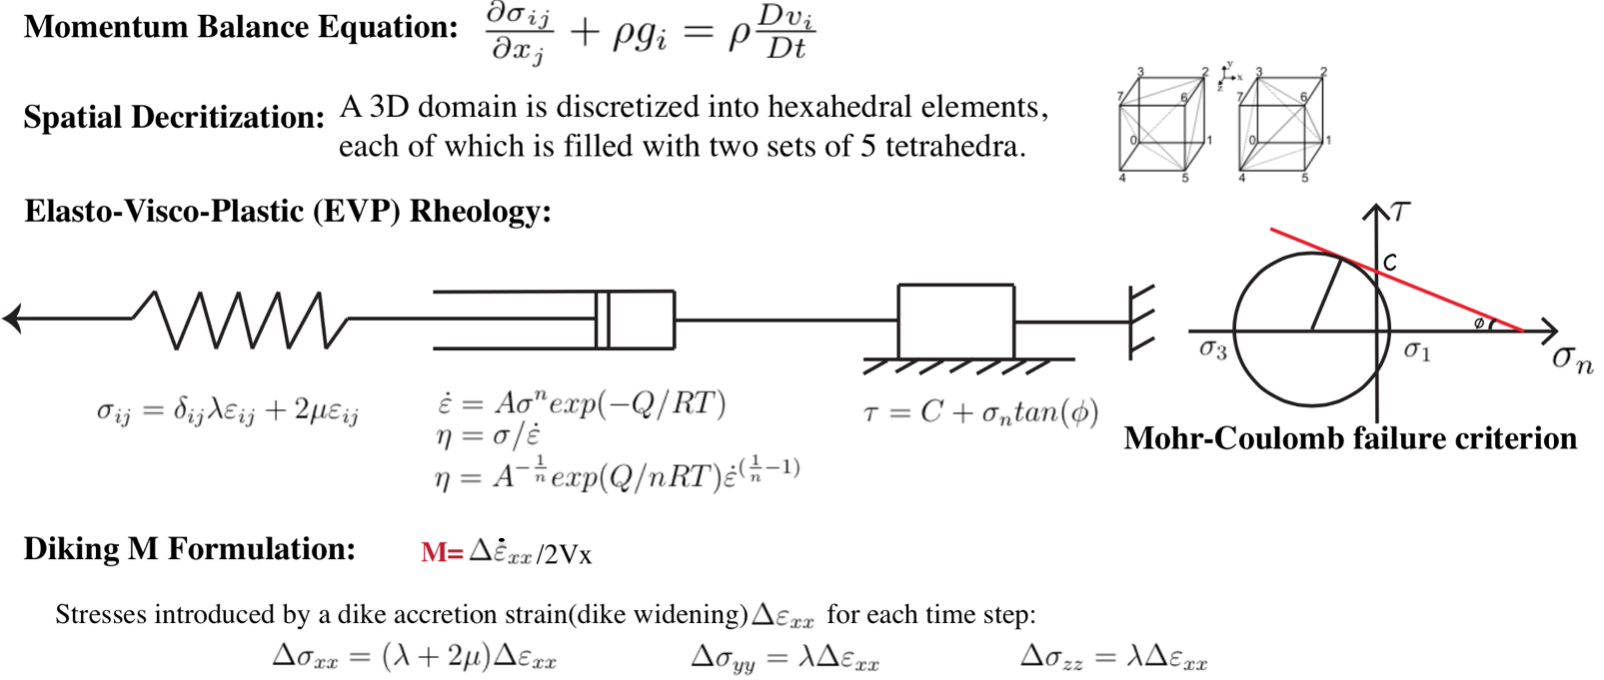
\includegraphics[scale=0.65]{fig_Methods7_2.png}
  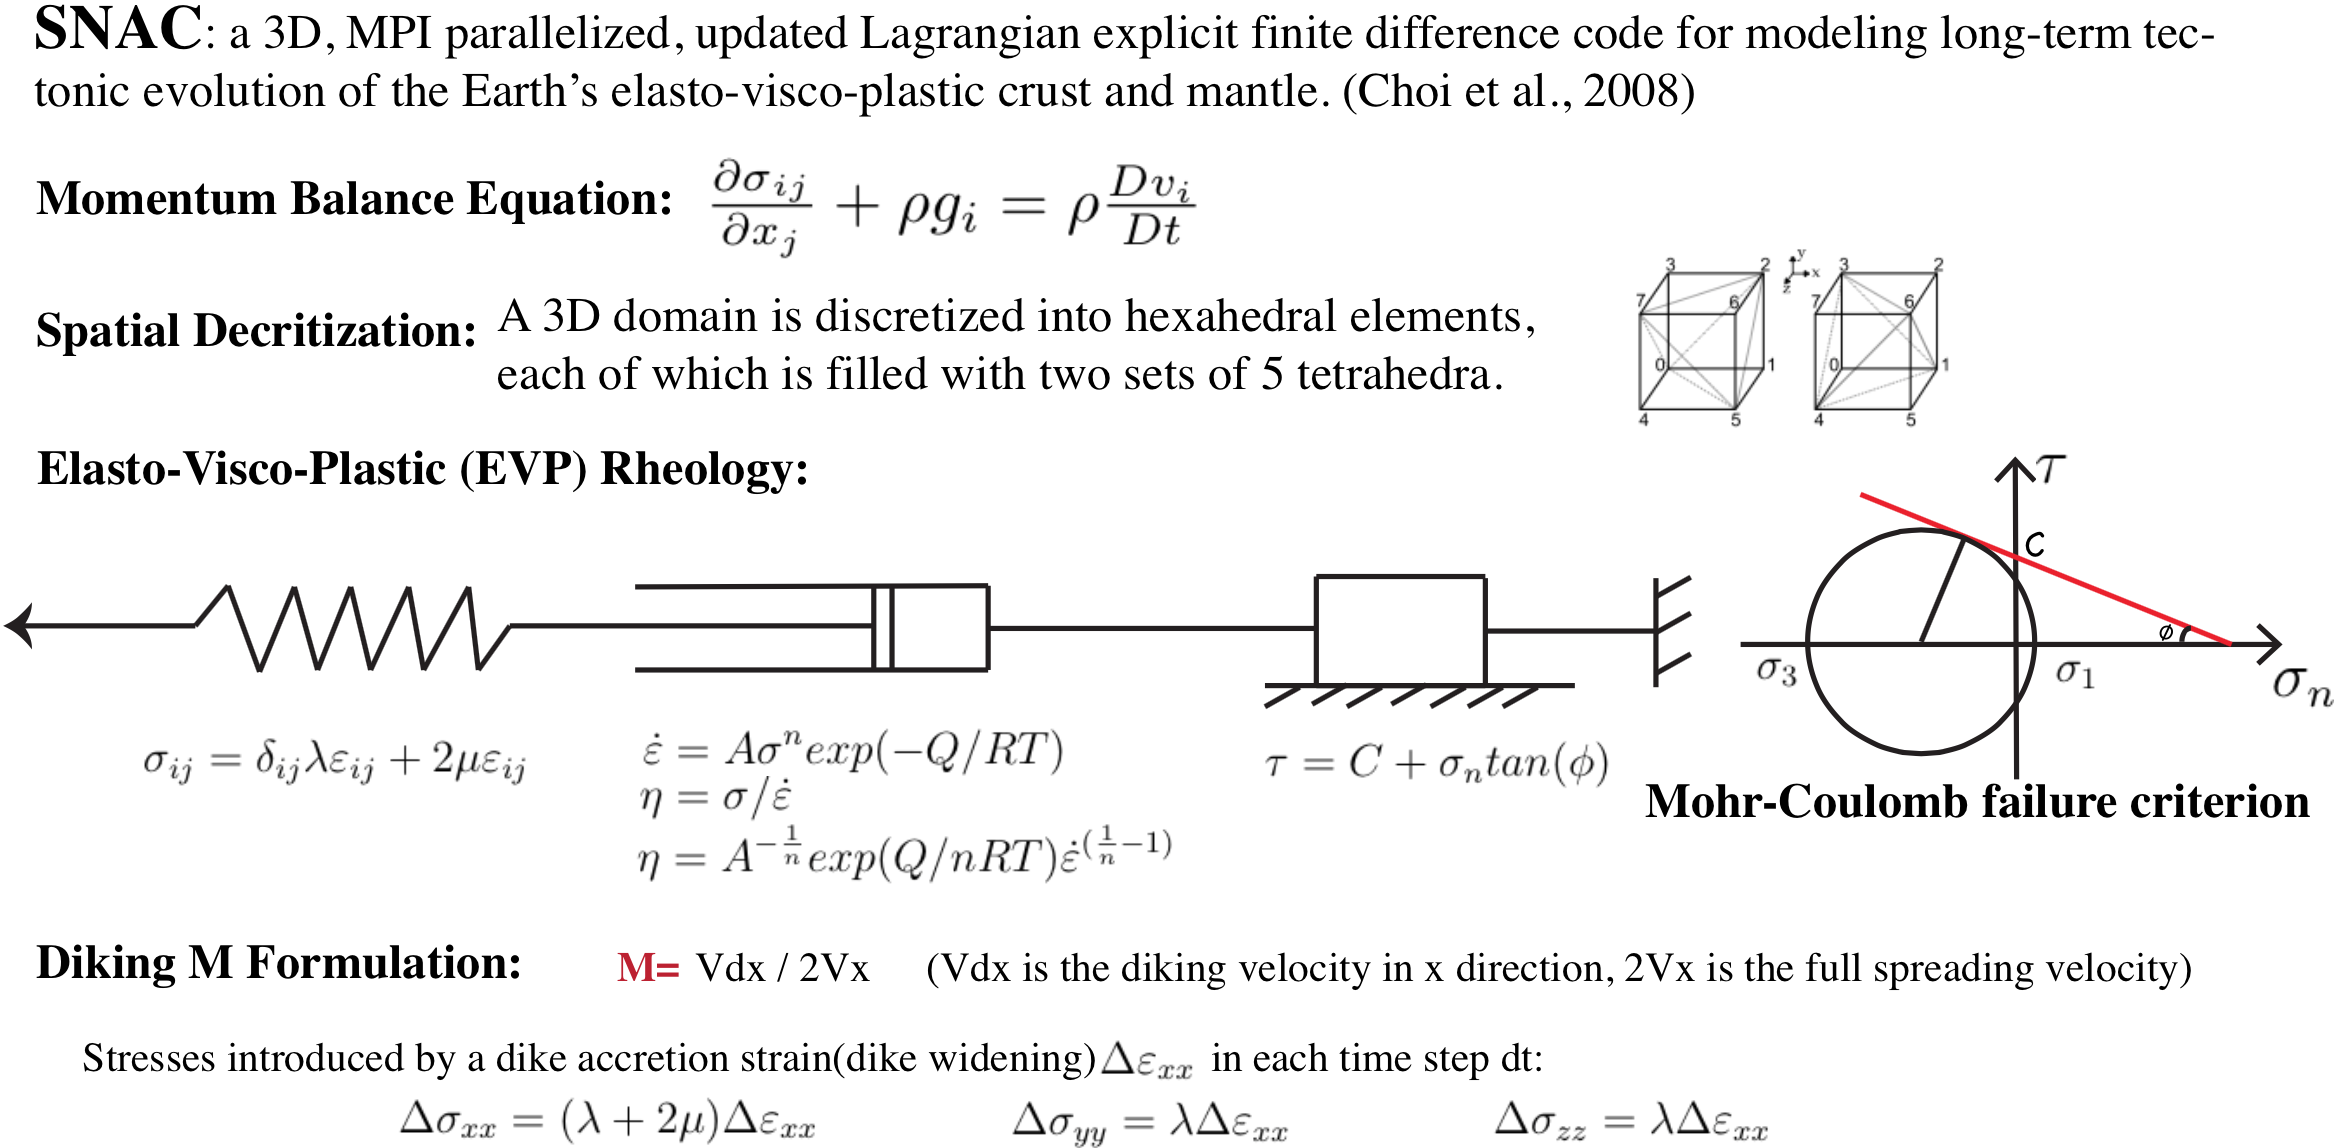
\includegraphics[width=1.0\textwidth]{fig_Methods7_3.png}
 \caption{\small{Essential components of the numerical method to be used for the proposed research}}
 \label{fig_Methods7_3}
\end{figure}

\subsection{Model Setup}
\add[XT]{Add a table for parameters in use.}
The 3D models has a geometry of (60km $\times$ 20km $\times$ 20km) in X, Y and Z axes respectively with a resolution of \change[EC]{dx$=1km$ (dx}{$dx$=1km ($dx$} is the \change[EC]{length scale for}{size of} each hexahedron element. \note[EC]{you might want to change the simbol to $\Delta x$ since $dx$ often represents infinitesimal amount.} \add[EC]{For comparison with the previous 2D models (e.g., Buck et al. 2005; Tuckholke et al., 2008), I also run} \remove[EC]{For }pseudo-2D models\change[EC]{,}{and} they have a geometry of ($60km \times 20km \times 1km$) in \change[EC]{X, Y and Z}{$x$, $y$ and $z$} axes respectively with a resolution of \change[EC]{dx$=0.5km$}{$dx=$0.5 km}. As shown in Figure~\ref{fig_Methods8_1}, \add[EC]{the initial} temperature \add[EC]{field} linearly increases from 0 \degree C at the top surface to 240 \degree C at the depth of 6 km, reflecting enhanced cooling due to hydrothermal circulation. Below 6 km, the temperature profile follows the semi-infinite half-space cooling model of moving plates \citep[e.g.,][]{Turcotte2002}. Two sides perpendicular to the $z$ coordinate axis are free-slip. The top surface has \remove[EC]{a} vertical traction\add[EC]{s} from water column\add[EC]{s}, of which height\add[EC]{s} \change[EC]{is}{are} locally determined as \change[EC]{4000-h(x,z)}{$4000-h(x,z)$} m, where \change[EC]{h(x,z)}{$h(x,z)$} is the topography at a location, \change[EC]{(x,z)}{$(x,z)$}. The bottom surface is supported by the Winkler foundation. Temperature is fixed at \annote[EC]{0\degree C}{As with other units, you'll have to decide whether to put a space between the number and the unit and stick to it.}  on the top surface and at 1300\degree C on the bottom surface. We \annote[EC]{will}{Also be consistent with the tense: i.e., consistently use past, present or future tense.} adopt the power-law rheology of dry diabase\citep[e.g.,][]{Kirby1987, Buck2005}. 

\begin{figure}[H]
 \centering
%  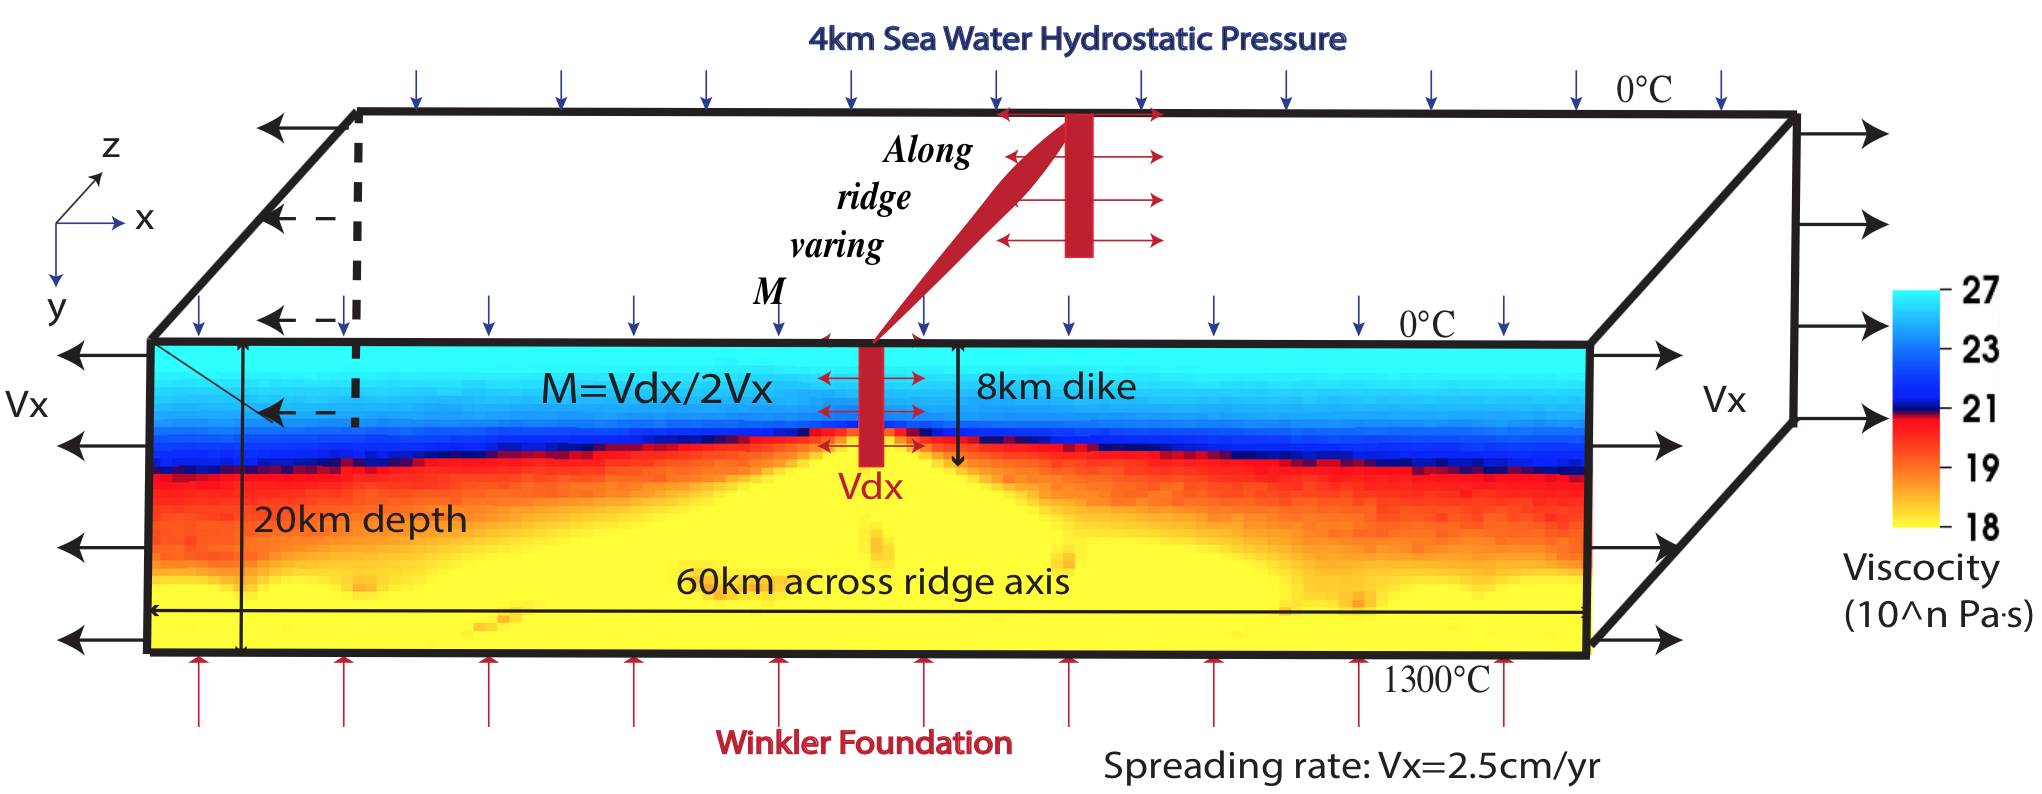
\includegraphics[scale=0.55]{fig_Methods8_1.png}
  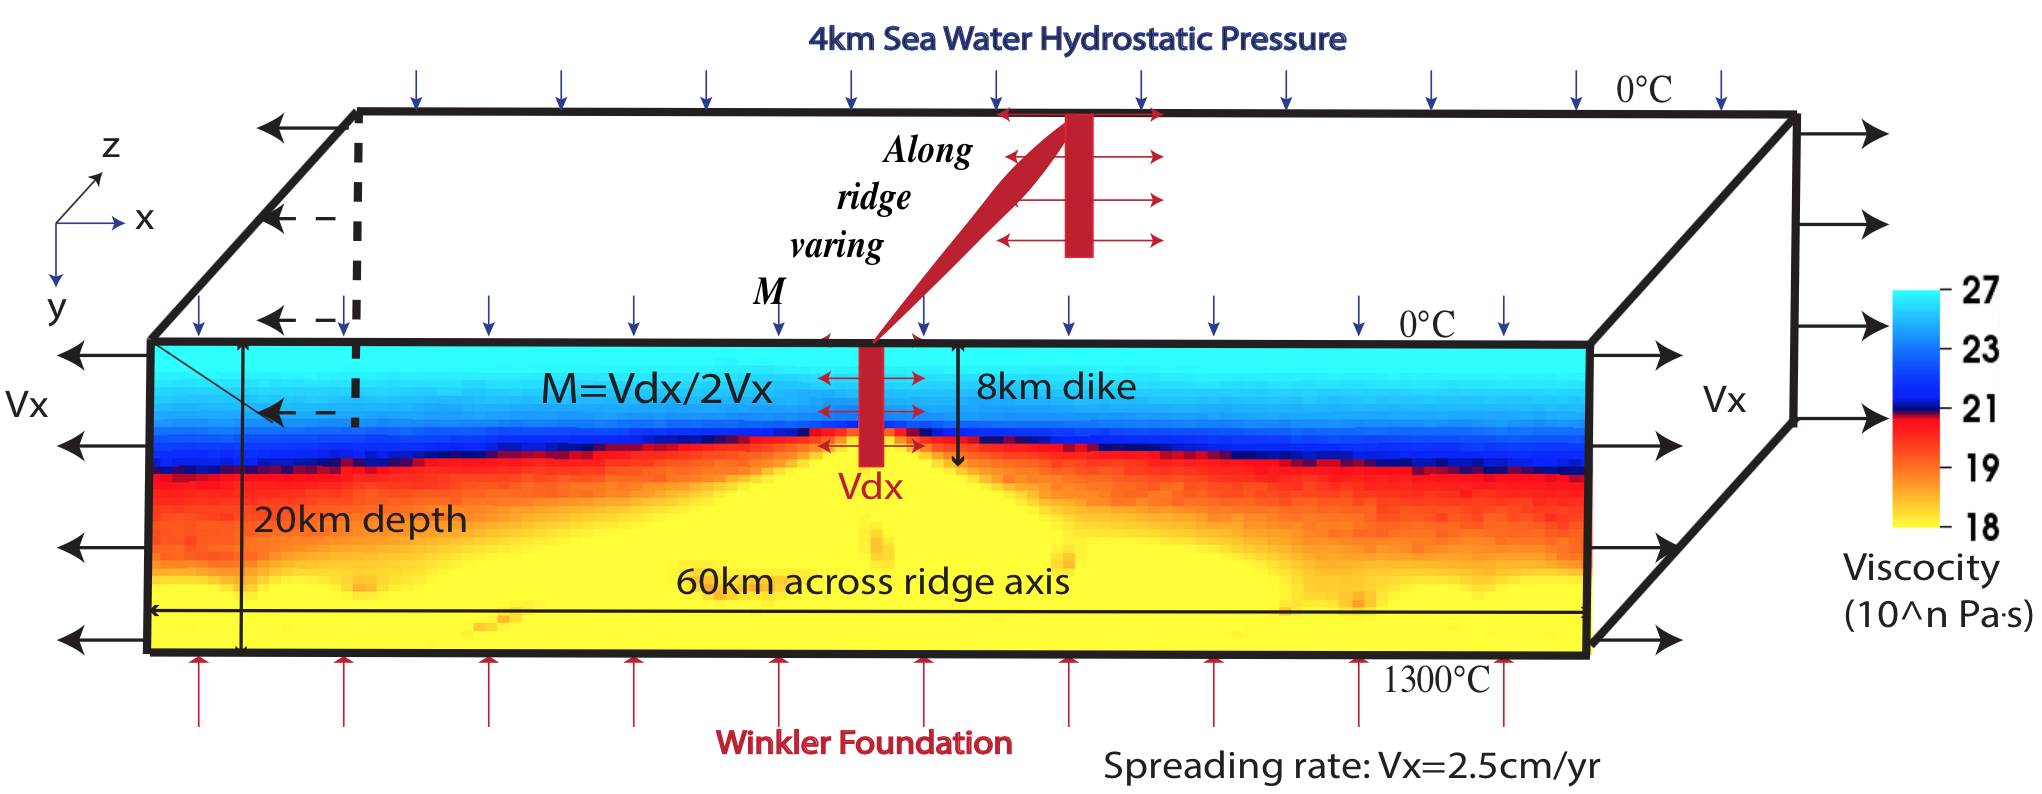
\includegraphics[width=1.0\textwidth] {fig_Methods8_1.png}
 \caption{\small Model setup}
 \label{fig_Methods8_1}
\end{figure}


\subsection{Parameters to control}
Although how to estimate the M values from observations \change[EC]{has not been well established}{is a subject of on-going research}, we do have constraints from a large dataset of bathymetry, gravity and seismic surveys as well as geological drilling. Generally, at slow spreading ridges, magma supplies mostly at the center of the ridge segment and decreases towards the end of the segment \citep{Tolstoy1993,Chen1999}. There is also evidence for shorter wavelength of 10 to 20 km discrete focus of magma accretion along the ridge axis \citep{Lin1990}. 

Based on these constraints, we can start considering only a few end-member scenarios of variations in M along the ridge axis. The variation in M is \change[EC]{parametrized in terms of the}{given in some simple} functional forms \change[EC]{(e.g.}{such as} \annote[EC]{discrete increment}{what is this? Piecewise constant?}, linear, sinus\change[EC]{u}{o}idal and square root\change[EC]{),}{.} \annote[EC]{its wavelength}{wavelength of what? A sinusoidal function?} (e.g. 10km, 20km and 40km) and the ranges of M (e.g. 0.2 to 0.8, 0.5 to 0.7 and 0.5 to 0.8). \note[EC]{The current writing gives an impression that you are going to make every possible combination of these. It is not true, right? I know you are planning to add a table of all the models but also state that what combinations of the geometric components you actually run.}

Preliminary pseudo-2D results show that the model behavior in faulting pattern is sensitive to the rate of strain weakening. Two cases of strain weakening are tested in this study. In one case (denoted as Type 1), cohesion linearly decreases from 44 MPa (denoted as $C_{i}$) to 4 MPa ($C_{e}$) for plastic strain accumulating from 0 ($\varepsilon_{p_{i}}$) to 0.1 ($\varepsilon_{p_{e}}$). It has a characteristic fault slip of 150 \change[EC]{meters}{m} for pseudo-2D models and 300 meters for 3D models\note[EC]{Explain why the values of the characteristic slip should be different.}. The other case (Type 2) assumes cohesion linearly decreasing from 44 MPa to 4 MPa for plastic strain accumulating from 0 to 0.33. In this case, the characteristic fault slip for Pseudo-2D models is 500 meters and for 3D models is 1km.
\note[EC]{don't see a need to start a new paragraph. So I deleted the new line.}
The characteristic fault slip \add[EC]{is defined as} $\Delta X_{c}=3 \times dx \times \varepsilon_{p_{e}}$ \note[EC]{how about $\Delta X_{c}=3 \, dx \, \varepsilon_{p_{e}}$?} \change[EC]{(}{, where} 3\add[EC]{$dx$ represents} \remove[EC]{is because} the thickness of the shear bands \add[EC]{which} is usually 2 to 4 times \remove[EC]{of the} \change[EC]{dx}{$dx$} \citep{Lavier2000})\change[EC]{ means w}{. W}hen $\Delta X_{c}$ amount of \change[EC]{displacement}{slip} takes place at the fault interface, the \change[EC]{C}{c}ohesion of the material at the faulting interface will decrease to $C_{e}$. In this way, under \add[EC]{the} same amount of $\Delta X_{c}$, models with different resolution should \change[EC]{behave in the same way in terms of strain weakening and}{produce the same} faulting patterns. 

